\documentclass[11pt, a4paper, german]{article}
\usepackage[german]{babel}%Deutsche Anf�hrungszeichen usw
\usepackage{pdfpages}%Einf�gen von pdfs
\usepackage{lmodern}%Schriftart
\usepackage{setspace}%Zeilenabstand
\usepackage[utf8]{inputenc}%Umlaute
\usepackage[T1]{fontenc}%Encoding Umlaute etc.
\usepackage{graphicx}%F�r das Einf�gen von Grafiken
\usepackage{placeins}%Ebenso
\usepackage{float}%Ebenso
\usepackage{subfigure}%Ebenso
\usepackage[bottom]{footmisc}
\usepackage{geometry}%Seitenlayout
%\geometry{
%	left=3cm,
%	right=2cm,
%	top=2cm,
%	bottom=2cm,
%	%bindingoffset=5mm
%}

\usepackage{booktabs}
\usepackage{hyperref}%f�r hyperrefs in pdf

\usepackage{tikz}
\usetikzlibrary{arrows,shapes,positioning,shadows,trees}
%%%%%%%%%%%%%%%%%%%%%%
\usepackage{bibgerm} %deutsches "und"
\usepackage{csquotes}
\usepackage{listings}
\usepackage{url}
\usepackage{etoolbox}
\appto\UrlBreaks{\do\a\do\b\do\c\do\d\do\e\do\f\do\g\do\h\do\i\do\j
	\do\k\do\l\do\m\do\n\do\o\do\p\do\q\do\r\do\s\do\t\do\u\do\v\do\w
	\do\x\do\y\do\z}
\usepackage[backend=bibtex,
style=authortitle,
giveninits=false,
citestyle=authortitle-ibid,
maxbibnames=3,
maxcitenames=2
]{biblatex}
\bibliography{Literatur}
%citestyle=authortitle-ibid
%%%%%%%%%%%%%%%%%%%%%%%%%%
%%%%%%%%%%%%%%%%%%%%%%%%%%
%%%%%%%%%%%%%%%%%%%%%%%%%%
%%%%%%%%%%%%%%%%%%%%%%%%%%
\title{Library Caprentry\\Konrad F\"orstner und Till Sauerwein\\Workshop April 2019}
\author{Notizen von Dina He\ss}
%%%%%%%%%%%%%%%%%%%%%%%%%%
\begin{document}
	
	%\doublespacing
	%\frontmatter
	%\setcounter{page}{0}
	%\includepdf[pages={1}, fitpaper=true]{title.pdf}
	%\cleardoublepage%leere Seite, sodass das n�chste auf ner ungeraden Seite beginnt
	\maketitle
	%\mainmatter
	\tableofcontents
	\cleardoublepage
	\thispagestyle{empty}
	\pagenumbering{roman}
	\newpage
	\pagenumbering{arabic}
%%%%%%%%%%%%%%%%%%%%%%%%%%%%%%%%%%%%%%%%%%%%%%%%
\section{Library Carpentry - Begriff}
Der Begriff Library Carpentry kommt von Software Carpentry. Dabei war die Idee, WissenschaftlerInnen spezifische IT-Skills für ihren Bereich an die Hand zu geben. Dabei ist wichtig, dass alle Vorgänge den folgenden Grundsätzen genügen. Sie sind
\begin{itemize}
	\item Reproduzierbar
	\item Transparent
	\item Nachvollziehbar (Tracking)
\end{itemize}
Aus Software Carpentry entwickelte sich Data Carpentry und verschmolz somit zu \emph{The Carpentries}. Schließlich entstand daraus 2014 auch Library Carpentry. 

Der Kurs soll als Startpunkt für Library Carpentry gesehen werden. Austausch ist wichtig! Anregung (Konrads Team): wöchentliche HackieHour. Ziel ist: 
\begin{itemize}
	\item Automatisierung, Optimierung von (wiederholbaren) Tasks und Prozessen
	\item Reproduzierbarkeit und Transparenz (nicht immer das Rad neu erfinden, nachnutzbar, nachvollziehbar)
	\item Gibt größere Handlungsfähigkeit, größeren Handlungsspielraum (warum eine teure Software kaufen, wenn man Software mit demselben Ziel mit offenen Methoden selbst und offen \emph{nachnutzbar} selbst machen kann -- kann Geld sparen!)
	\end{itemize}
%%%%%%%%%%%%%%%%%%%%%%%%%%%%%%%%%%%%%%%%%%%%%%%%%%
\section{Unix-Shell}
Alternatives (zu anderen, vgl. Mac Terminal) Interface/Schnittstelle zum Betriebssystem. Wir nutzen die Version \emph{Bash} einer solchen Shell. Die Windows-Version davon heißt Git bash. 
\begin{quote}
	Die Shell ist mächtig.\\
	Sie kann zum Kopieren, Verschieben und Kombinieren mehrerer Dateien (auch gleichzeitig und in großer Menge) verwendet werden. 
\end{quote}
\subsection{Erste Schritte}
Zu unterscheiden zwischen den primären Befehlen (nach dem \$-Zeichen), Argumenten (Flags) und Parametern.\\ 
$\star$ Hier handschriftliche Notizen einfügen\\

\noindent\texttt{ls --help} listet mögliche Befehle/Eingaben und allgemeine Hilfe. 

\noindent\texttt{mkdir firstdir}. Mit \texttt{TAB} kann man Befehle bzw. Parameter auto-vervollständigen. \texttt{ls -a} listet nun alles auf, was da ist. In einem leeren Ordner stehen da die Optionen \texttt{./} bezeichnet das aktuelle Verzeichnis, \texttt{../} bezeichnet das darüberliegende Verzeichnis (Eltern-Ordner).\\ 

\emph{Faulheit ist eine Tugend!}\\

\noindent Um den Großeltern aufzurufen ist auch der Befehl \texttt{cd ../..} möglich.\\

\noindent Es handelt sich hierbei um relative Pfade. \texttt{\$ cd /c/Users/Dina/Desktop/Library Carpentry 2019/shell-lesson} ist dabei der absolute Pfad. Um dabei ins Home-Directory zu kommen nutzt man die Tilde, bzw. ein simples \texttt{tilde} bringt mich ins Home-Directory.\\

Mit den Pfeil-hoch und Pfeil-runter Tasten kann man vorher genutzte Befehle aufrufen und ggf. erneut verwenden.  

Durch \texttt{STRG+r} kann ich ein Muster eingeben, um ähnliche Befehle wieder aufzurufen (nacheinander wieder mit \texttt{STRG+r}. Mit \texttt{STRG+c} kann man das wieder abbrechen -- auch Programme stoppen).\\

\noindent Mit \texttt{STRG+a} kann man im Befehl an den Anfang, mit \texttt{STRG+e} ans Ende und mit \texttt{STRG+k} nach dem Cursor löschen, mit \texttt{STRG+u} alles vor dem Cursor löschen.\\

\subsubsection{Dateiendungen betrachten}
\texttt{json} -- JavaScript-Ding (.js ausführbar). Alle in shell-lesson befindlichen Dateien sind letztendlich Textdateien (Plaintext), die man mit Texteditoren bearbeitet werden können. 

\subsection{Plaintext-Dateien lesen}
Der Befehl \texttt{cat} gibt den Text einer Plaintext-Datei aus und gibt es als Rückgabe zurück. \texttt{head} gibt nur die ersten 10 Zeilen aus. Äquivalent dazu der Befehl \texttt{tail} mit den letzten 10 Zeilen. 

\noindent\texttt{head -n 20 name.txt} gibt die ersten 20 Zeilen aus.\\

Mit dem Befehl \texttt{less} können Daten strukturiert angezeigt werden (mit \texttt{q} kommt man wieder raus). Mit \texttt{less -S datei.tsv} kann man das auch noch als Tabelle anzeigen lassen. 

Fazit: Wir können die Dateien anschauen, sie ausgeben, Teile ausgeben und Dateien strukturiert ausgeben. Mit
\texttt{head -n 5 datei1.txt datei2.txt} kann man auch zwei ausgeben (erste 5 Zeilen hier). Nervig wirds so bei mehr Dateien. \texttt{head -n h *txt}. Dabei steht der * repräsentantiv für mehrere Dinge. Dies nennt man auch Globbing (wiederholbar für weitere solche Dinge). Es können alle möglichen Teile auch kombiniert werden: \texttt{ls 2014*31*tsv}. Ähnlich zu etwa der Arbeit mit regulären Ausdrücken.

Mit \texttt{ls -1} kann man übrigens die Liste als 1 Spalte ausgeben. 

\subsection{Konvention}
Datumsangaben immer 2019-04-02 (ISO 8601), inkl. Bindestriche (darf man weglassen, sollte man aber nicht). Überlegt auch immer, wie man die Dateien nennt. 

\subsection{Dateien verschieben und umbenennen etc.} 
\texttt{mkdir dateiname} -- Verzeichnis erstellen\\
\texttt{mv dateiname.txt neuername.txt} -- Datei umbenennen. Beachte hier: kontextabhängiges Verhalten:\\
\texttt{mv dateiname.txt verzeichnisname/} -- verschiebt in ein anderes Verzeichnis.\\
\texttt{mv dateiname.txt firstdir/neuername.txt} -- verschieben und umbenennen.\\
\texttt{mv anderesverzeichnis/dateiname.txt .} -- zurückschieben ins aktuelle Verzeichnis.\\
\texttt{cp dateiname.txt neuedatei.txt} -- erstellt eine Kopie der ersten Datei mit dem Namen neuedatei.txt

\subsection{Datenformate}
Betrachten mal .html oder .json .tsv (Tabellen) usw. 

\subsection{For-Schleifen/For-loops}
Konzept, das in allen Programmiersprachen zu finden ist. Prinzip: wende eine Aktivität auf mehrere Dinge an. 

\texttt{touch} ändert Zeitstempel oder erstellt Datei (falls noch nicht existiert). Angenommen, wir wollen einen Befehl wie \texttt{cp} mehrfach anwenden auf alle Dateien, die einem Muster genügen. $\rightarrow$ For-Schleife.

\subsubsection*{Syntax einer For-Schleife}
\noindent\texttt{FOR\dots IN Menge}\\
\texttt{DO\dots}\\
\texttt{done}.\\

Im \textbf{Beispiel} also:\\
\texttt{for FILE in \{a.pdf, b.pdf, c.pdf\}}\\
\texttt{do}\\
\texttt{cp \$ FILE \$ FILE-Backup}\\
\texttt{done}\\

Beachte: In FILE werden hier die Dateinamen abgelegt. Ferner ist hier anstelle einer Menge in Unix-Shell einfach eine Liste anzugeben. \\

\begin{figure}[h]
	\centering
	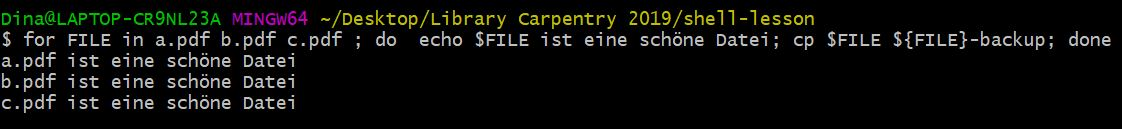
\includegraphics[width=\linewidth]{bild2}
	\caption{}
	\label{fig:bild1}
\end{figure}

Dabei ist \texttt{echo} ein Befehl zur Ausgabe (besser: \texttt{printf})

\subsubsection{Schöne Befehle}
\texttt{wc} -- Wordcount\\
\texttt{wc -l} -- Anzahl Zeilen\\
\texttt{rm} -- löscht eine Datei\\
\texttt{rm -i *txt} -- entfernt alle txt-Dateien, fragt aber vorher.\\

\begin{figure}[h]
	\centering
	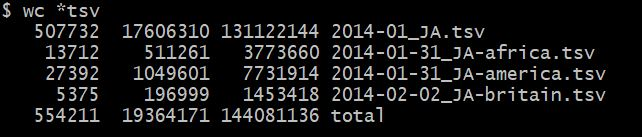
\includegraphics[width=0.7\linewidth]{bild1}
	\caption{}
	\label{fig:bild2}
\end{figure}

Eine Datei mit den Ausgaben erstellen geht durch \texttt{>}: siehe Abb. \ref{fig:bild3}

\begin{figure}[h]
	\centering
	
\includegraphics[width=0.7\linewidth]{bild3}
	\caption{}
	\label{fig:bild3}
\end{figure}

Da die Länge an erster Stelle steht (als Zahl), kann ich die ausgegebene Liste sortieren nach Länge. Siehe Abb. \ref{fig:bild4}

\begin{figure}[h]
		\centering
	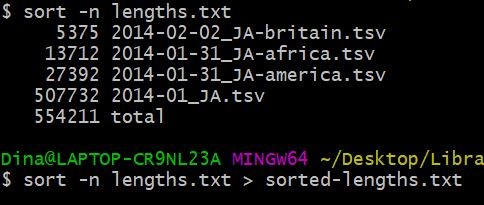
\includegraphics[width=0.7\linewidth]{bild4}
	\caption{}
	\label{fig:bild4}
\end{figure}

Man kann dann durch \texttt{\$ head -n 1 sorted-lengths.txt} die Datei mit der kürzesten Länge angeben. 

\subsubsection{Pipes}
Das Zeichen \texttt{|} sagt: der Output aus links wird direkt in rechts reingesteckt (Abb. \ref{fig:bild5}).

\begin{figure}[h]
	\centering
	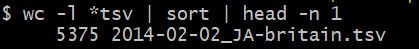
\includegraphics[width=0.7\linewidth]{bild5}
	\caption{}
	\label{fig:bild5}
\end{figure}

\subsubsection*{Beispiel}
Ich kann also einen gescannten Text erst in eine OCR-Software, das Ergebnis in eine Texttdatei schreiben und diese durch ein Indexierungsprogramm jagen. Mit einem Befehl. \\

Beachte: Dateien werden mit \texttt{>} einfach überschrieben. Nicht aber mit \texttt{>>}.\\

\texttt{grep -c} mit count. nicht nur Ausgabe. 

\begin{figure}[h]
	\centering
	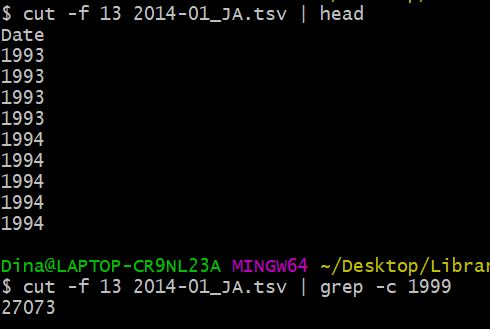
\includegraphics[width=0.7\linewidth]{bild8}
	\caption{}
	\label{fig:bild8}
\end{figure}
 
 Man kann mit einer Handvoll weniger Befehle schöne Sachen zusammen bauen. Man kann solche einfachen Analysen machen oder Dinge automatisieren. Ich wende Aktionen auf viele Dateien an. 
 Zum Thema Reproduzierbarkeit: Skripte. 
 
 \subsection{Shell-Skripte}
 Auch Shell-Skripte sind wiederum Plaintext-Dateien, die eine Liste von Befehlen enthält. Eine Art \emph{Kochrezept zum Ausführen}. 
 Arbeite mit dem Editor nano. Dieser öffnet/generiert eine Datei namens count\_lines.sh (siehe Abbildungen 7f.). Damit wir erkennen, dass es ein Shell-Skript ist, enden wir mit .sh. In den gängigen Editoren spricht man von Syntax-Highlighting (Färben bestimmter Wörter und Zeichen nach ihrer Funktion). (Nano-Befehle: Strg+o zum Speichern, Strg+x um den Editor zu verlassen).
 \begin{figure}[h]
 	\centering
 	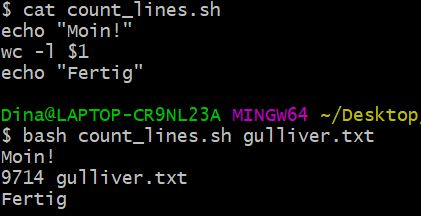
\includegraphics[width=0.7\linewidth]{bild9}
 	\caption{}
 	\label{fig:bild9}
 \end{figure}
  Beachte nun: Mit \texttt{\$1} kann ich Variablen einlesen (vorher stand da \texttt{*txt}). 
  
  $\Rightarrow$ Programmierung mit Variablen! Morgen können wir die Änderungen (hier von Einfach zu Komplexer) mit Git tracken. 
  
  \section{Python}
  Python ist eine der am stärksten wachsenden und populärsten Sprachen. Sie ist vergleichsweise einfach zu lernen und sehr mächtig. Python ist zudem frei verfügbar und hat inzwischen eine sehr große Community. 
  
  Merke: Jupyter Notebook. Könnte die Zukunft des Wissenschafts-Outputs sein (statt klassische Aufsätze), da man Code, Kommentar und ausgeführten Code (z.B. Bilder) kombinieren kann. Durch \# kann auch hier ein Kommentar eingesetzt sein.
  
  False und True als Boolesche Variablen
  
  Container anlegen \texttt{variablenname $=[1, 2, 3]$}. Die Zahl an der ersten Stelle aufrufen kann man dann durch \texttt{variablenname$[0]$}.Beachte, um das zu tun, die erste Zeile vorher \emph{ausgeführt} werden muss. Funktion: \texttt{len} für die Länge eines Containers/einer Variable. (Bei Help -- Keyboard Shortcuts gibrs ein paar Befehle für die Faulen).
  
  Mit \texttt{variablenname.upper()} wird der String darin in Großbuchstaben ausgegeben. Analog mit \texttt{lower} klein. Mit ? lassen sich Infos zum jeweiligen Objekt anzeigen. 
  
  \subsection{For-Schleifen}
  Vergleiche ab hier auch das 1. Jupyter-Notebook
  
  \subsection{Built-in-functions}
  \noindent\texttt{print()}\\
  \texttt{len()}\\
%%%%%%%%%%%%%%%%%%%%%%%%%%%%%%%%%%%%%%%%%%%%%%%%
	%\clearpage
	%\section{Literatur}
	%\printbibliography[heading=none]
	%\clearpage
	%\input{Anhang}
	
\end{document}
